\section{Performance and Experimental Challenges}
\label{sec:performance_and_challenges}

\subsection{Performance of the spherical harmonics analysis on 0{\nbb} decay and $^{8}$B events.}

Comparison of $S_0$ and $S_1$ distributions between 0{\nbb} decay and
$^{8}$B events is shown in Fig.~\ref{fig:S_vs_energy}. There is a
noticeable separation between the signal and background. We also note
that in the energy range of interest, the $S_l$'s do not strongly
depend on the energy deposited in the detector, which makes them
reliable discriminators at the end point of the 0{\nbb} decay energy
spectrum. This makes the information about the event topology complimentary to
the energy measurements.

\begin{figure*}[h]
\centering
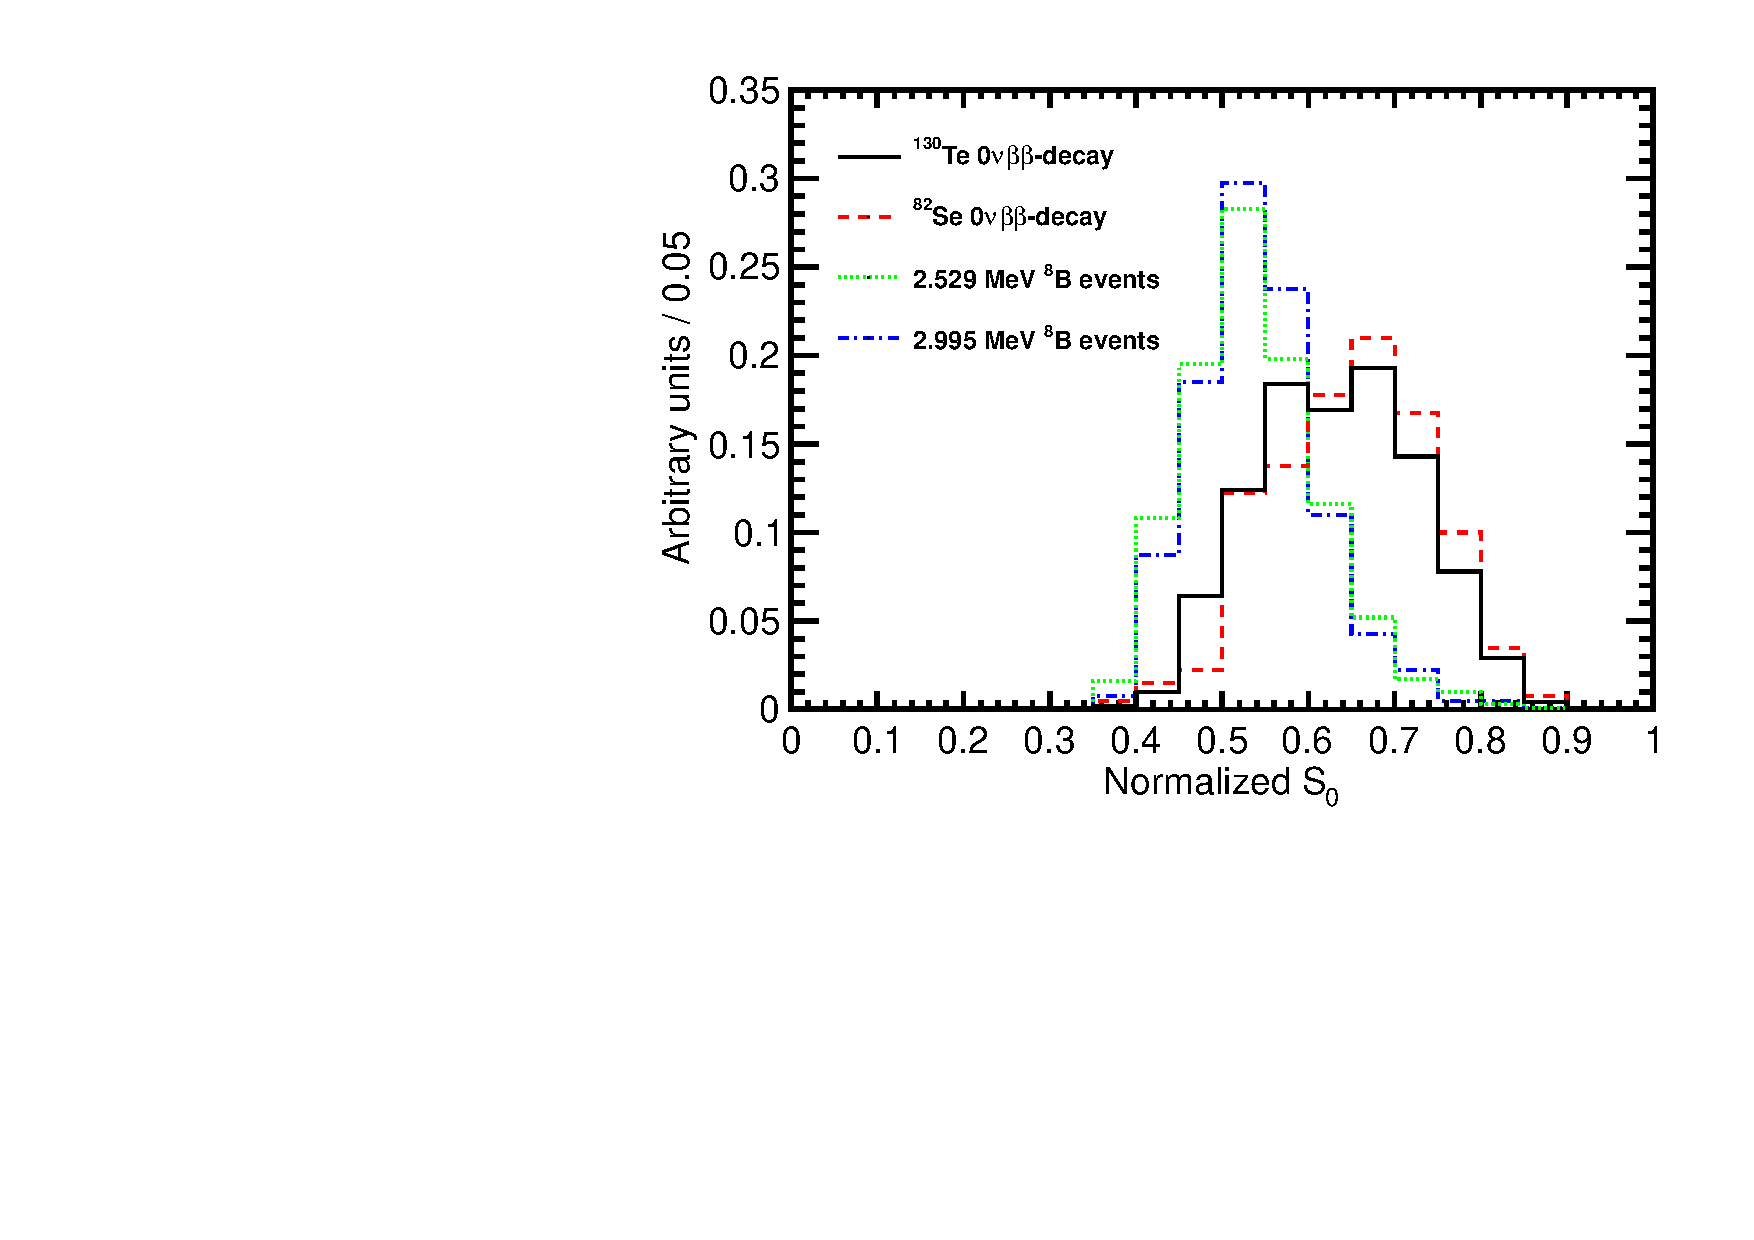
\includegraphics[width=0.49\textwidth]{hS0.pdf}
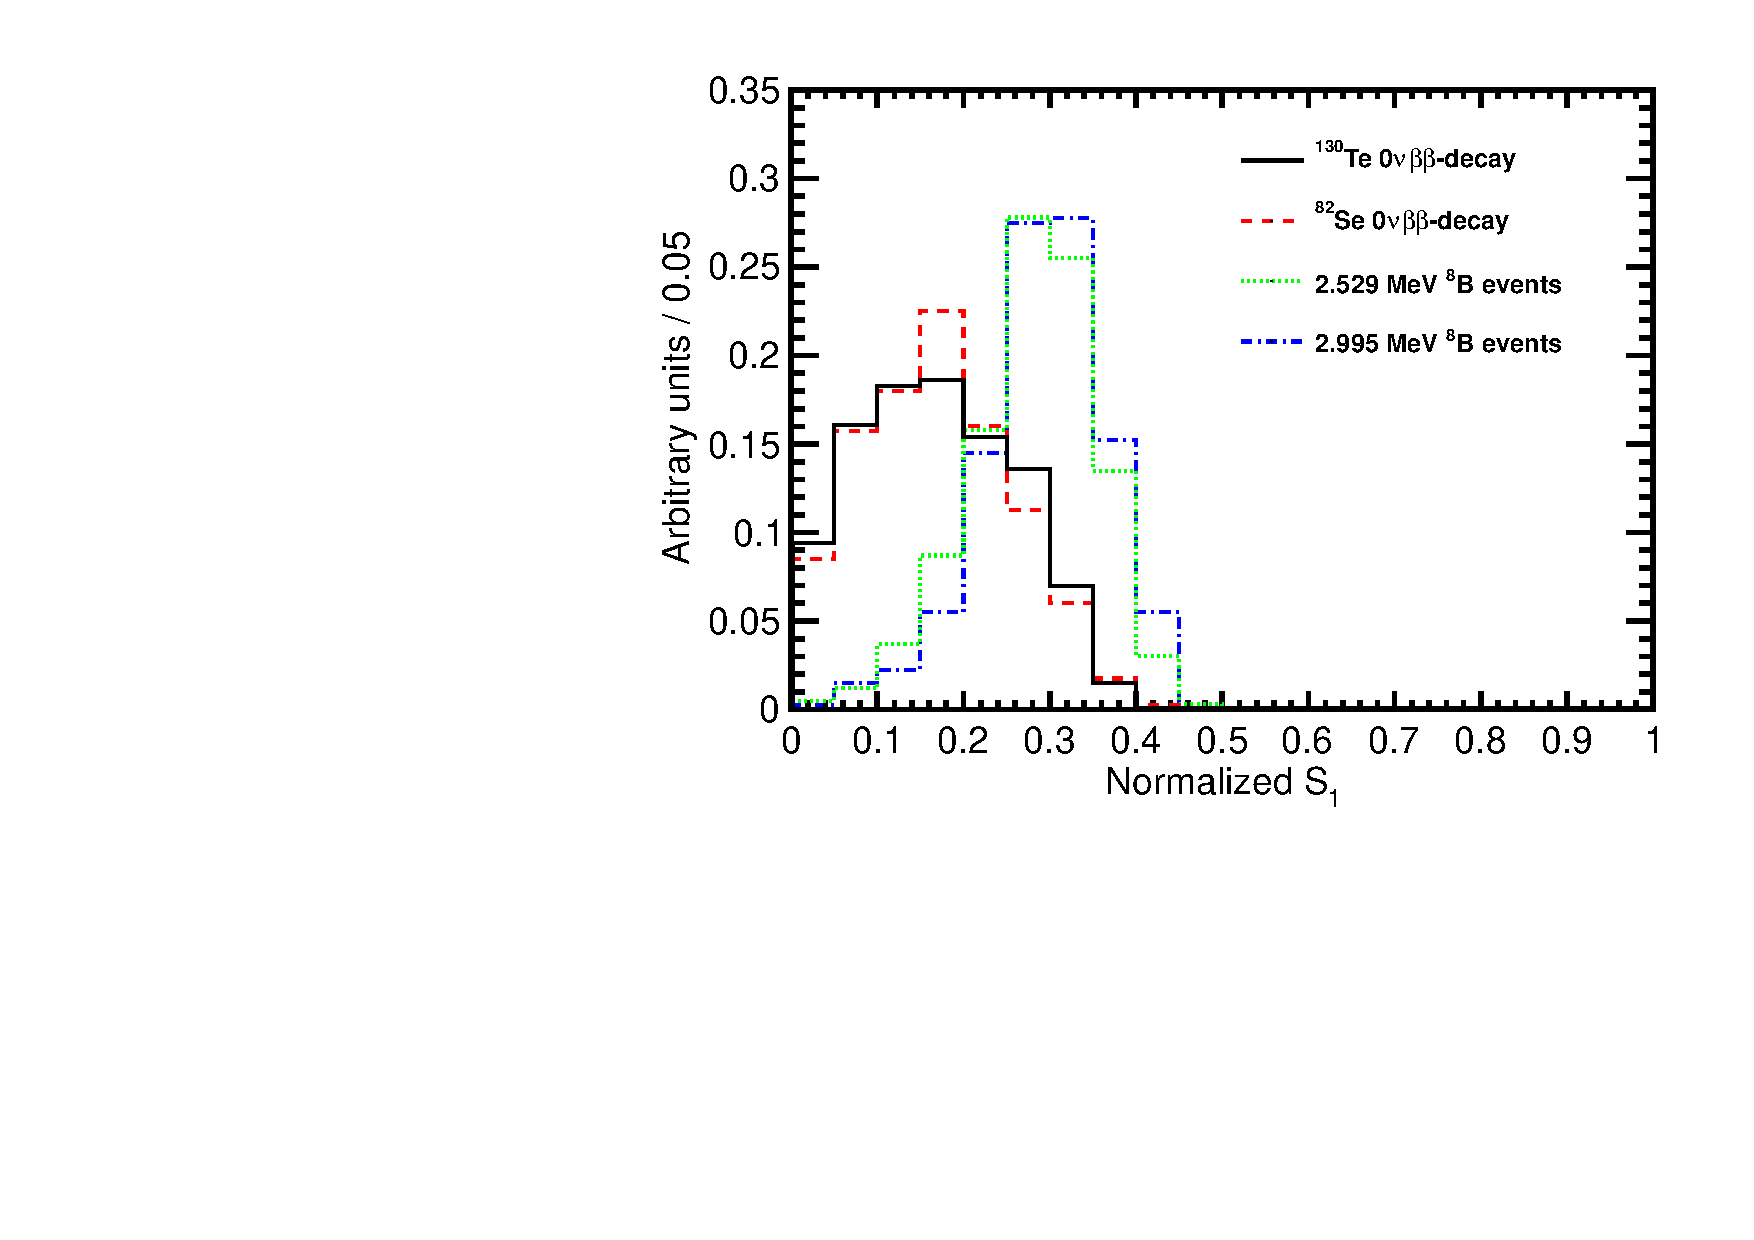
\includegraphics[width=0.49\textwidth]{hS1.pdf}
\caption{$S_0$ (\emph{left}) and $S_1$ (\emph{right}) distributions
  for events with two different event topologies and total kinetic
  energy. $^{130}$Te, $^{82}$Se 0{\nbb} decay, 2.529 MeV and 2.995 MeV
  events are compared. The simulation is done for events with the
  vertex in the center of the detector. $^{8}$B events are implemented
  as 2.529~MeV or 2.995~MeV electrons with initial direction along
  $x$-axis. Perfect vertex reconstruction - true vertex position is
  used. Time cut of 33.5~ns on the photon arrival time is applied.}
\label{fig:S_vs_energy}
\end{figure*}

Figure~\ref{fig:SL_Te_33p5ns_center} shows separation between
$^{130}$Te signal and $^{8}$B background events simulated at the
center of the detector. True values of the vertex position and time are
used. Also, a time cut of 33.5~ns on the photon arrival time is applied to
separate Cherenkov and scintillation light. Most of the discrimination
between signal and background comes from $S_0$ and $S_1$. In the
following, $S_2$ and $S_3$ are not used to separate $^{130}$Te and
$^{8}$B events (though $S_2$ and $S_3$ are helpful for separation of
  $^{130}$Te signal from $^{10}$C background. See Appendix.). The
scatter plot of $S_2$ vs $S_3$ is shown here for completeness.

In order to optimize the separation between $^{130}$Te signal and $^{8}$B
background, a linear combination of $S_0$ and $S_1$, $S_{01}$, is
used. A linear fit, $S_0$ = $A \times S_1 + B$, of the 2-dimensional $S_0$
vs $S_1$ scatter plot is performed as shown in
Fig.~\ref{fig:SL_Te_33p5ns_center}.  This 2-dimensional
distribution then is projected onto the fitted line. {\bf A little bit of
  math here to quantitatively describe $S_{01}$ via $S_0$ and $S_1$:}
A new coordinate frame is obtained by rotating the original
$S_0$-$S_1$ frame with the angle $\theta$ obtained from the fit:
$tan(\theta)$=$A$. A transformation, $S_{01} = S_1 \cdot cos(\theta) +
S_0 \cdot sin(\theta)$, defines the $S_{01}$ variable. The bottom plot in Fig.~\ref{fig:SL_Te_33p5ns_center} 
shows the performance of $S_{01}$ to separate $^{130}$Te signal and $^{8}$B
background events. A fit to this distribution can be done to optimize the
discrimination power for a particular experimental setting.

We refrain from quantitative estimates on the improvements in sensitivity
to 0{\nbb} decay searches using this method of spherical harmonics as a
reliable estimate would require a dedicated analysis taking into
account all the details of a particular experiment.

\begin{figure*}[h]
  \centering
  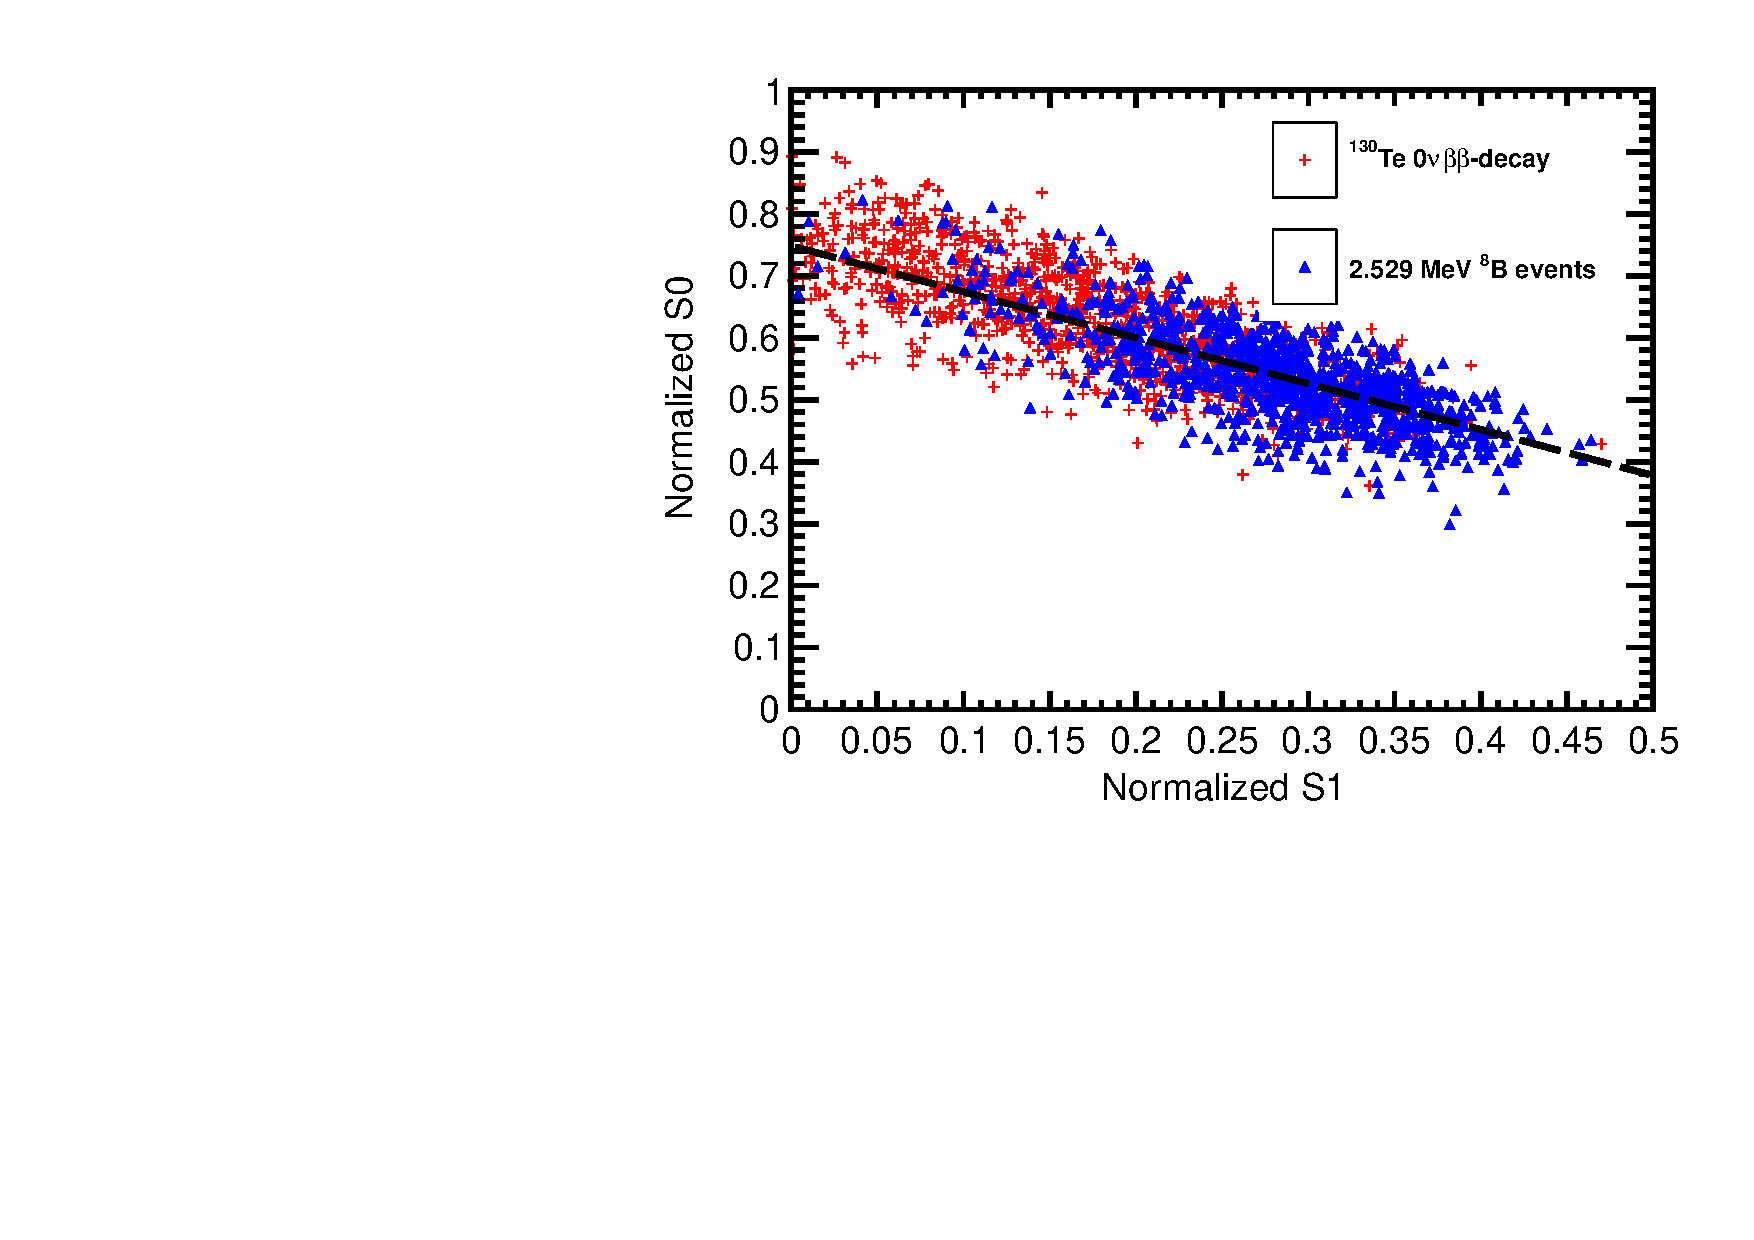
\includegraphics[width=0.49\textwidth]{hS0vsS1_Te130_1el_allLight_VtxSmear0cm_VtxShiftX0cm_33p5ns_center.pdf}
  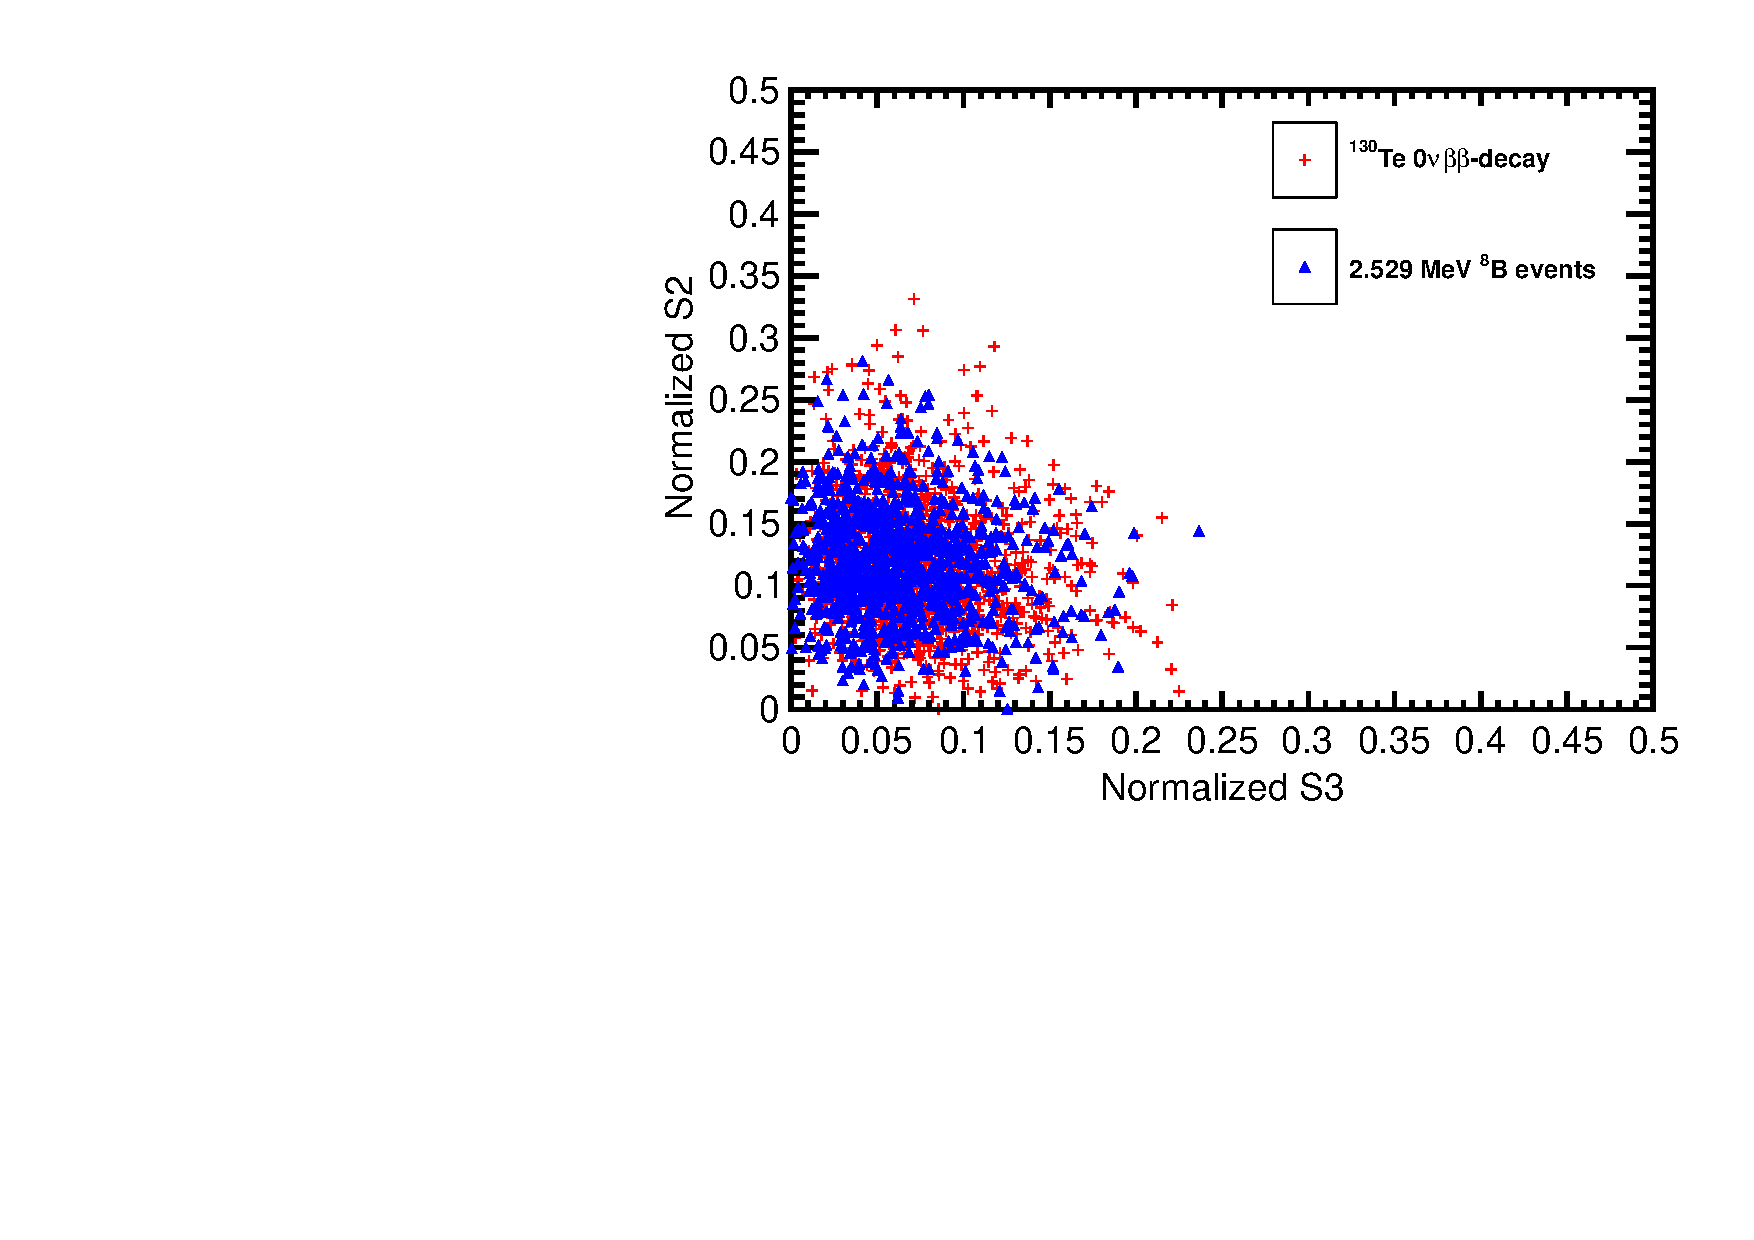
\includegraphics[width=0.49\textwidth]{hS2vsS3_Te130_1el_allLight_VtxSmear0cm_VtxShiftX0cm_33p5ns_center.pdf}
  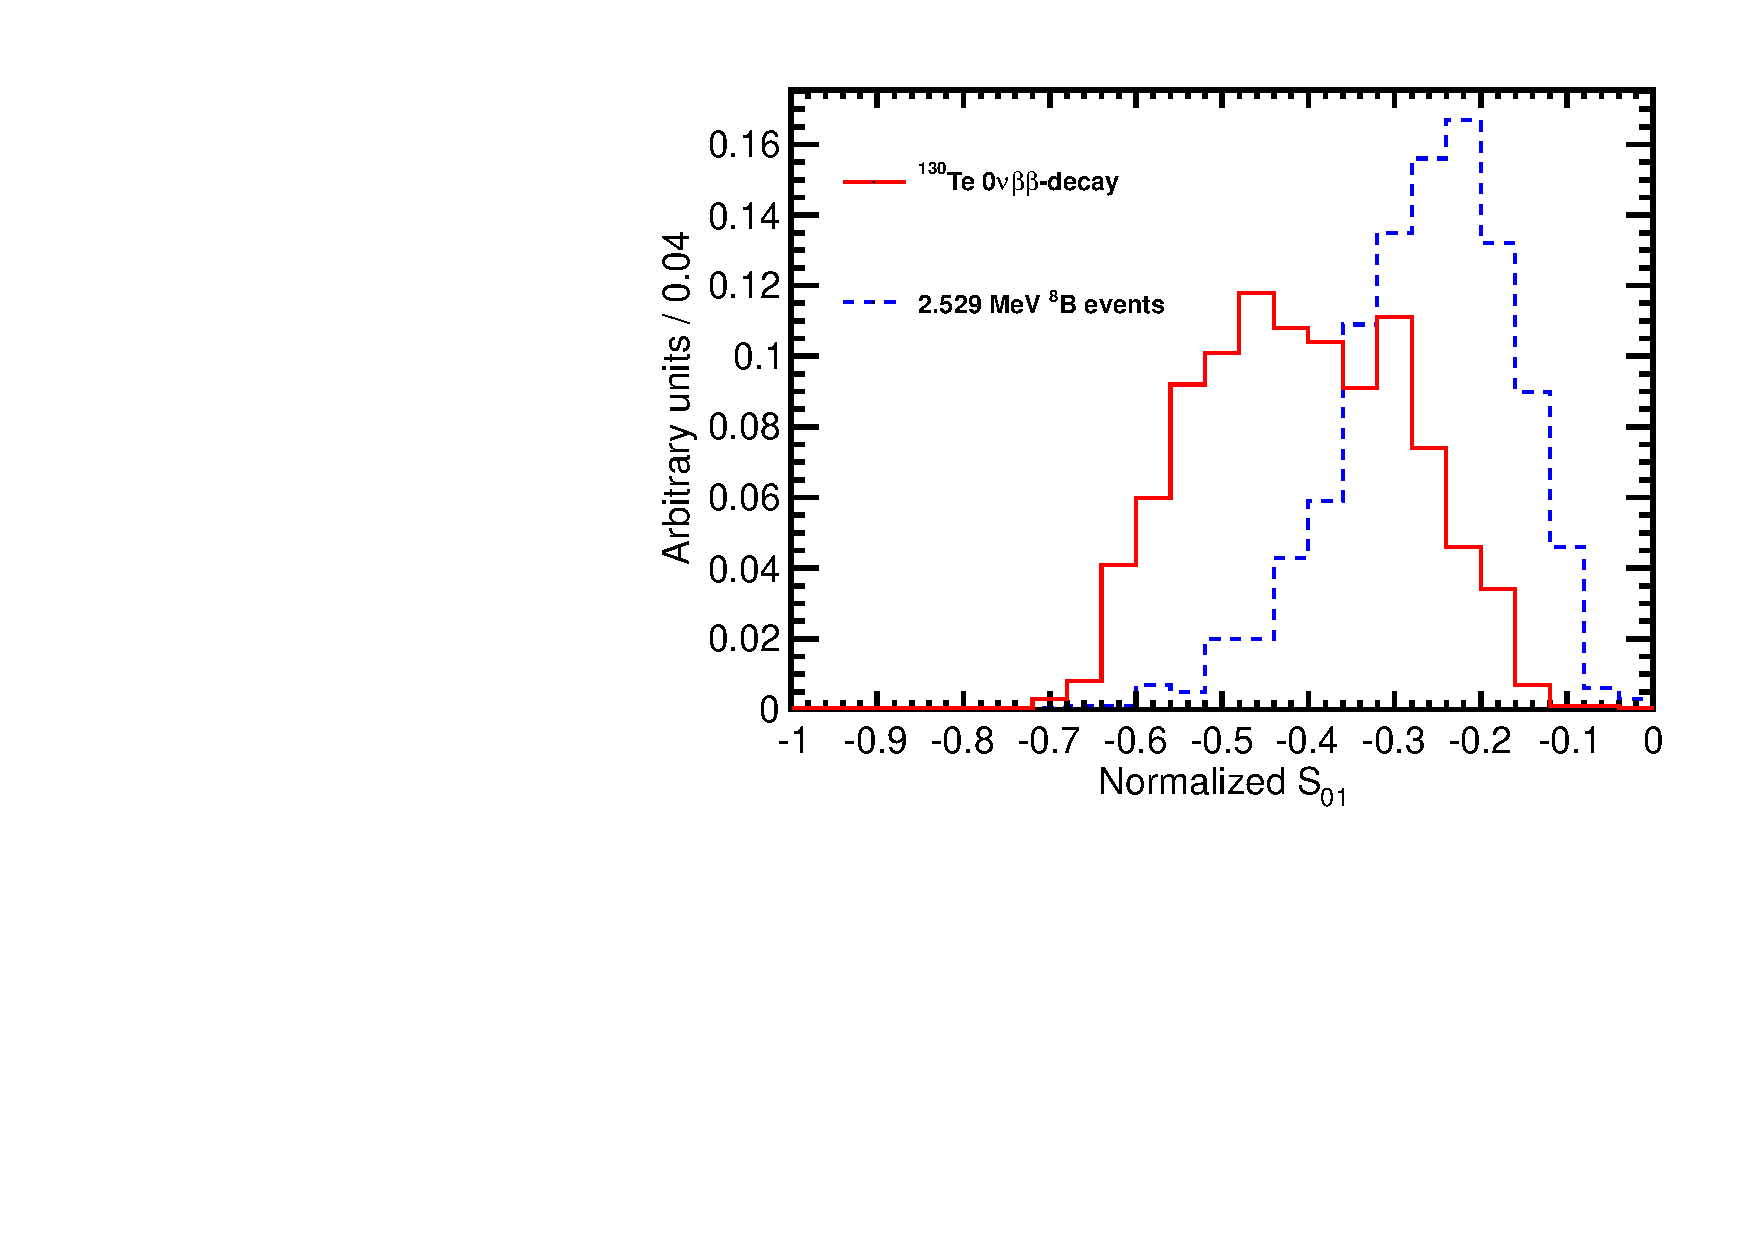
\includegraphics[width=0.9\textwidth]{hS01_allLight_VtxSmear0cm_VtxShiftX0cm_33p5ns_center.pdf}
  \caption{Spherical harmonics comparison between $^{130}$Te 0{\nbb}
    decay signal ($Q=2.529$~MeV) (\emph{red}) and $^{8}$B solar
    neutrinos background (\emph{blue}) for 1000 simulated events
    originated at the center of the sphere. $^{8}$B events are
    implemented as 2.529~MeV electrons with initial direction along
    $x$-axis. Perfect vertex reconstruction - true vertex position is
    used. Time cut of 33.5~ns on the photon arrival time is
    applied. \emph{Top left:} $S_0$ versus $S_1$ scatter plot. Black
    dotted line is a linear fit of these 2D histograms. Variable
    $S_{01}$ is defined as a projection of 2D distribution onto this
    linear fit. \emph{Top right:} $S_2$ versus $S_3$ scatter
    plot. \emph{Bottom:} $S_{01}$ distribution for the signal and
    background.}
\label{fig:SL_Te_33p5ns_center}
\end{figure*}


\subsection{Experimental challenges}

So far only events at the center of the detector have been
considered. In this section we discuss performance of the spherical
harmonics analysis for events distributed within the fiducial volume
of the detector taking into account finite resolution on vertex
position reconstruction.

The absolute cut (e.g., 33.5~ns) on the photon arrival time for central events relies on the fact that, within the uncertainty on electron track length, all photons travel for the same distance before  reaching the surface of the detector. 
PEs with early measured time correspond mostly to Cherenkov photons because of the delay in the scintillation process and longer wavelength of the Cherenkov light. 

When the vertex is not at the center, a uniform absolute time cut on the photon
arrival time is no longer effective in the selection of Cherenkov
photons. In the case of an off-center vertex, there could be a situation when even significantly delayed scintillation photons reach the side of the detector that is
closer to the vertex much earlier than Cherenkov photons traveling to
the opposite side of the detector. Therefore, the time cut has to take into account the total distance traveled to each PMT by each individual photon.

We found that a relative time cut defined as $\Delta t=t^{phot}_{measured} -
t^{phot}_{predicted}<$1~ns selects photons with a sufficient fraction being
Cherenkov photons. However two factors reduce the Cherenkov/scintillation light separation when this relative time cut is applied.

One reduction in the light separation comes from chromatic dispersion. The predicted time, $ t^{phot}_{predicted}=l/v^{phot}$, depends on the total distance, $l$, traveled by the photon and the velocity of the photon, $v^{phot}$.  Since the wavelength information is not available for a given PE, we must use an average index of refraction of n=1.53 and define the photon velocity as $v^{phot} = c/n$. This uncertainty on the photon velocity due to chromatic dispersion reduces the separation between scintillation and Cherenkov light. The other reduction in the light separation comes from the uncertainty in the reconstructed vertex position. This uncertainty leads to an uncertainty in the photon's total distance traveled and ultimately to a reduction in the Cherenkov/scintillation separation power.

When the whole fiducial volume of the detector is considered only the relative time cut can be used. Therefore, the effectiveness of the spherical harmonics analysis in separating of 0{\nbb} decay and $^{8}$B events is reduced. To demonstrate performance of the spherical harmonics analysis in a  more realistic experimental settings we define the fiducial volume within our detector as $R<3$~m and  simulate $\Te$ $\vbb$ signal and $\B$ background events with vertices uniformly distributed within that fiducial volume.

Figure~\ref{fig:SL_Te_SmearX0cm_momDT1ns_rndVtx_3p0m} compares the spherical harmonics for the signal and background events within the fiducial volume. Perfect vertex reconstruction is used in order to isolate the effect due to chromatic dispersion.   {\bf Don't understand this fragment: (to be compared with central events shown in Fig.~\ref{fig:SL_Te_33p5ns_center}).} Next generation LS detectors may be able to recover theses losses due to chromatic dispersion by choosing liquid scintillators with a more narrow emission spectrum (e.g. see Ref~\cite{LS_narrow_emission}).

\begin{figure*}[h]
  \centering
  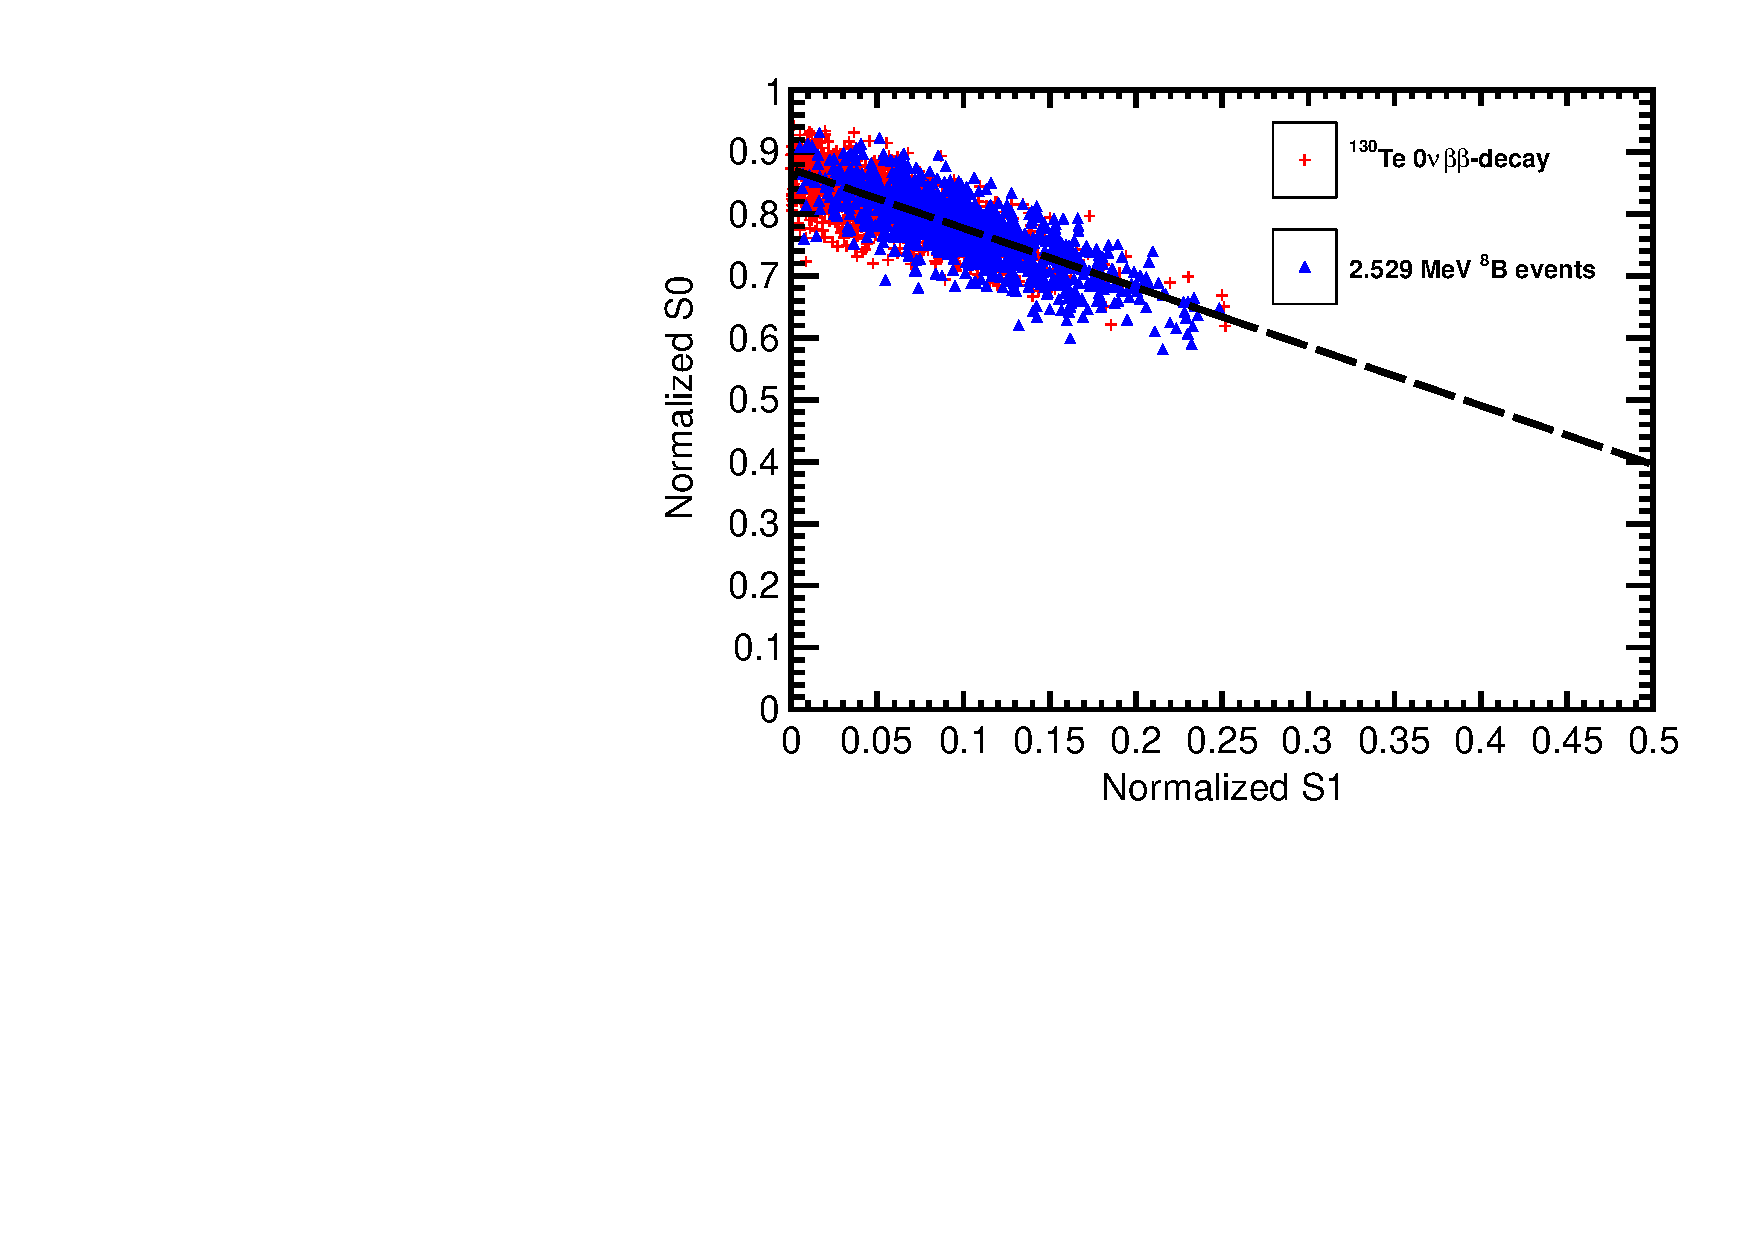
\includegraphics[width=0.49\textwidth]{hS0vsS1_Te130_1el_allLight_VtxSmear0cm_VtxShiftX0cm_momDT1p0ns_rndVtx_3p0mSphere.pdf}
  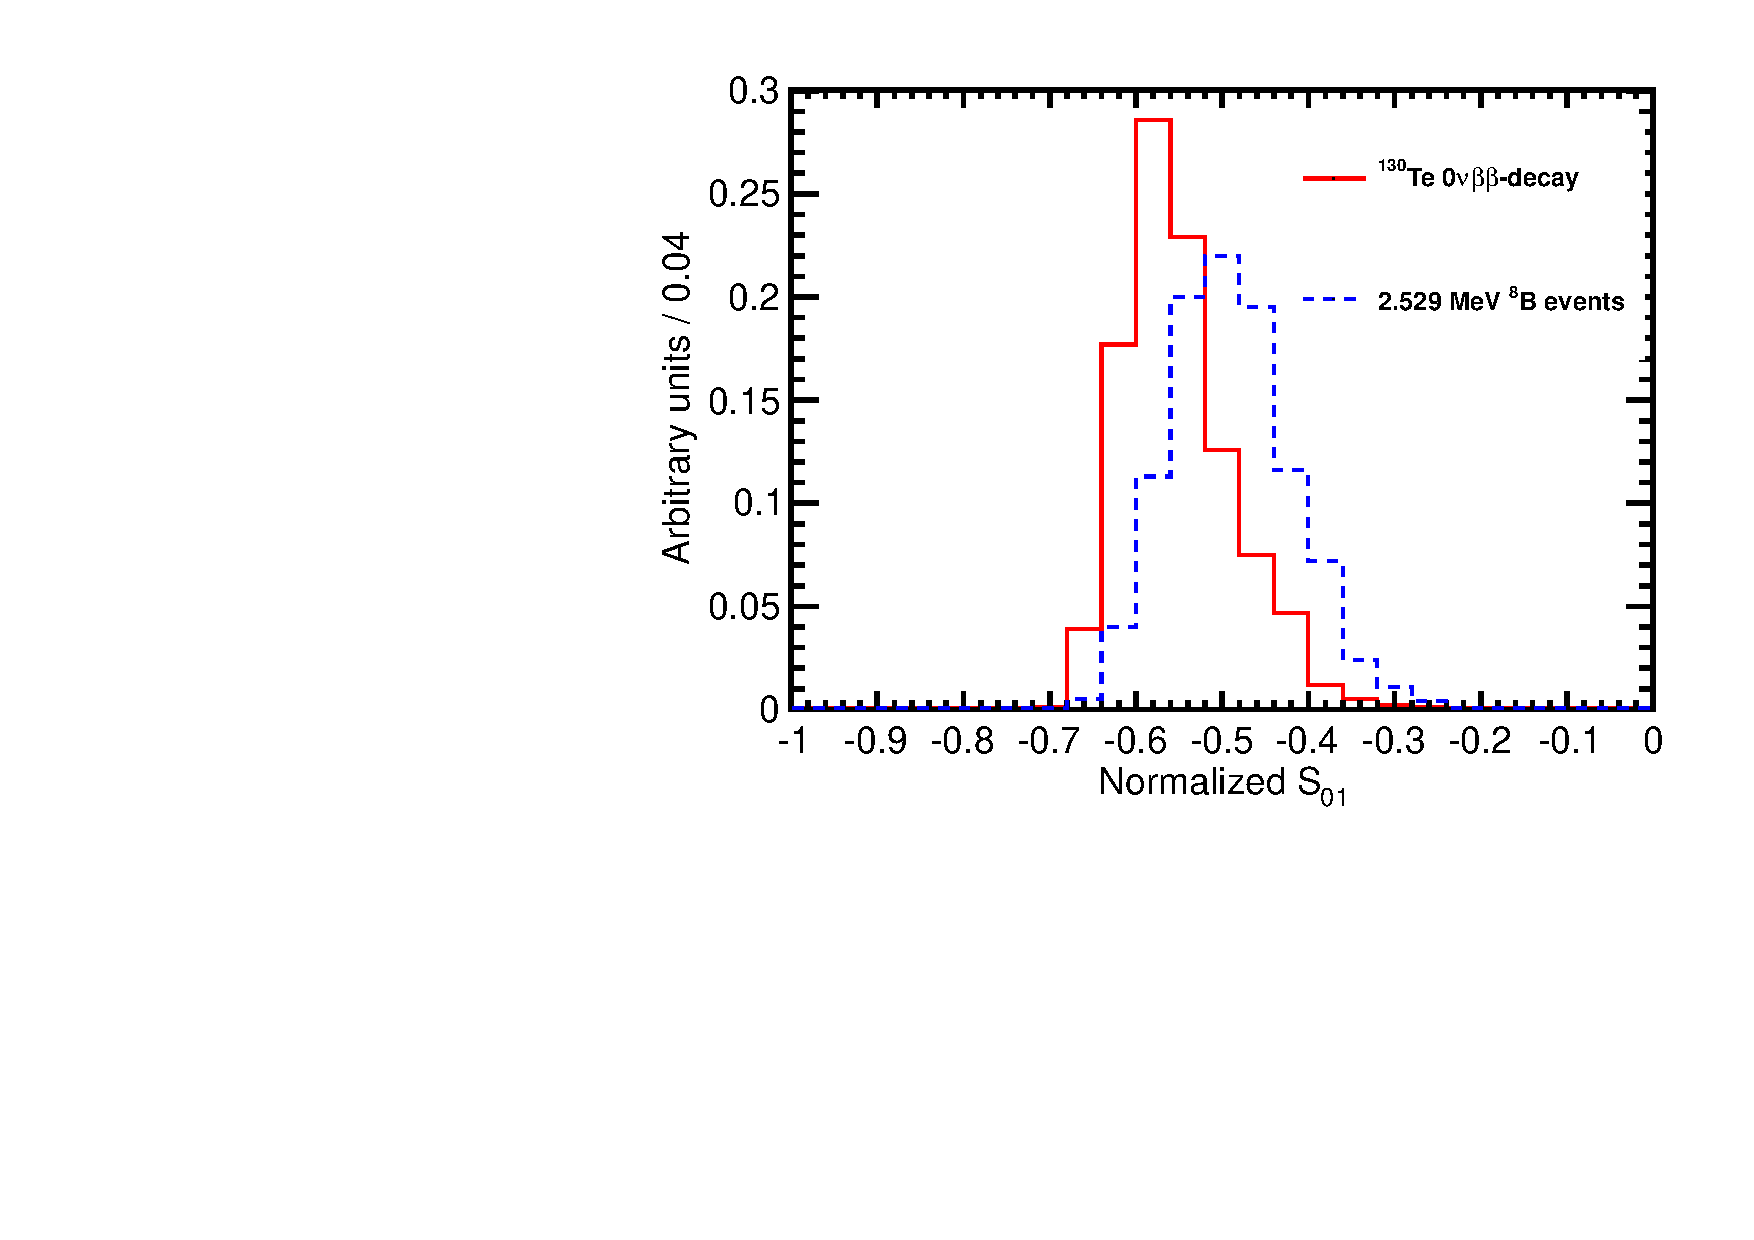
\includegraphics[width=0.49\textwidth]{hS01_allLight_VtxSmear0cm_VtxShiftX0cm_momDT1p0ns_rndVtx_3p0mSphere.pdf}
  \caption{Spherical harmonics comparison between $^{130}$Te 0{\nbb}
    decay signal ($Q=2.529$~MeV) (\emph{red}) and $^{8}$B solar
    neutrinos background (\emph{blue}) for 1000 simulated
    events.Verticies are uniformly distributed within the fiducial
    volume, $R<3$~m. $^8$Be events are implemented as 2.529~MeV
    electrons with the initial momentum direction uniformly
    distributed within 4$\pi$ solid angle. Perfect vertex
    reconstruction - true vertex position is used. \emph{Left:} $S_0$
    versus $S_1$ scatter plot. Black dotted line is a linear fit of
    these 2D histograms. Variable $S_{01}$ is defined as a projection
    of 2D distribution onto this linear fit. \emph{Right:} $S_{01}$}
  \label{fig:SL_Te_SmearX0cm_momDT1ns_rndVtx_3p0m}
\end{figure*}


Imprecise knowledge of the vertex position due to finite resolution is
the second factor affecting performance of the spherical harmonics
analysis. The vertex resolution not only reduces Cherenkov/scintillation light separation but it also affects the uniformity of the scintillation light distribution in the early PE sample.

Small deviations in vertex reconstruction cause a large effect
on the $S_0$ and $S_1$ distributions for the single electron event topology.
For the vertices shifted along the direction of the electron track the relative time cut $\Delta t$
reduces the uniformity of the scintillation light distribution. The
$\Delta t$ cut selects more forward emitted photons in the case when
the reconstructed vertex is shifted to the direction opposite to the
electron momentum. This enhances the forward region populated by Cherenkov
photons and causes a more asymmetric photon distribution that moves $S_1$ to higher values.  The opposite occurs for the case where the reconstructed vertex is shifted in the direction along the electron
momentum. Here, the time cut selects more backward emitted photons and counter balances the forward region populated by Cherenkov
photons leading to a more symmetric photon distribution and smaller values of $S_1$.

Figure~\ref{fig:SL_Te_SmearX3cm_momDT1ns_rndVtx_3p0m} shows the performance of the spherical harmonics analysis for events after taking into account a 3~cm vertex reconstruction resolution, applied uniformly within the fiducial volume. Since the goal of this paper is to introduce spherical harmonic analysis we do not perform a full vertex reconstruction and only apply smearing to the simulated vertex position using a Gaussian distribution with sigma of 3~cm on $x$, $y$, and $z$ coordinates. 

\begin{figure*}[h]
  \centering
  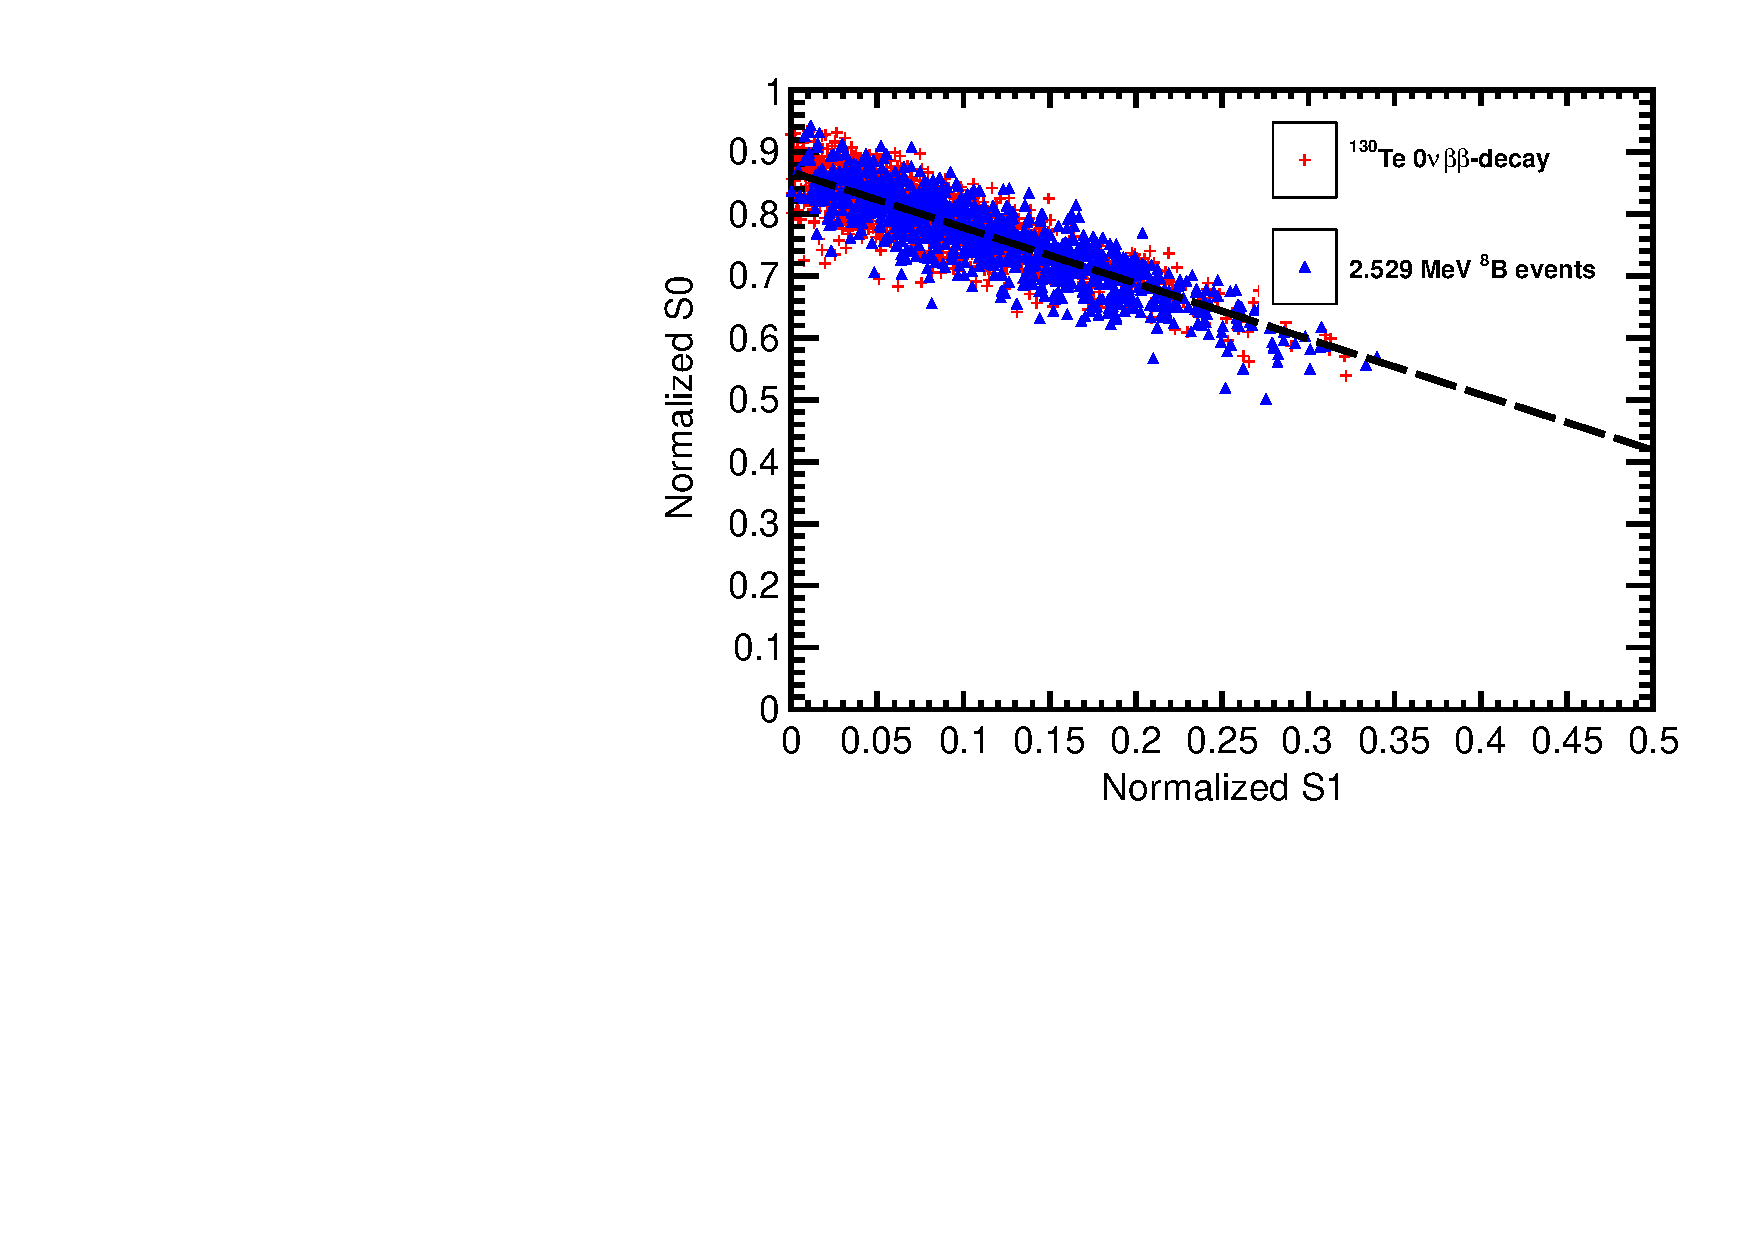
\includegraphics[width=0.49\textwidth]{hS0vsS1_Te130_1el_allLight_VtxSmear3cm_VtxShiftX0cm_momDT1p0ns_rndVtx_3p0mSphere.pdf}
  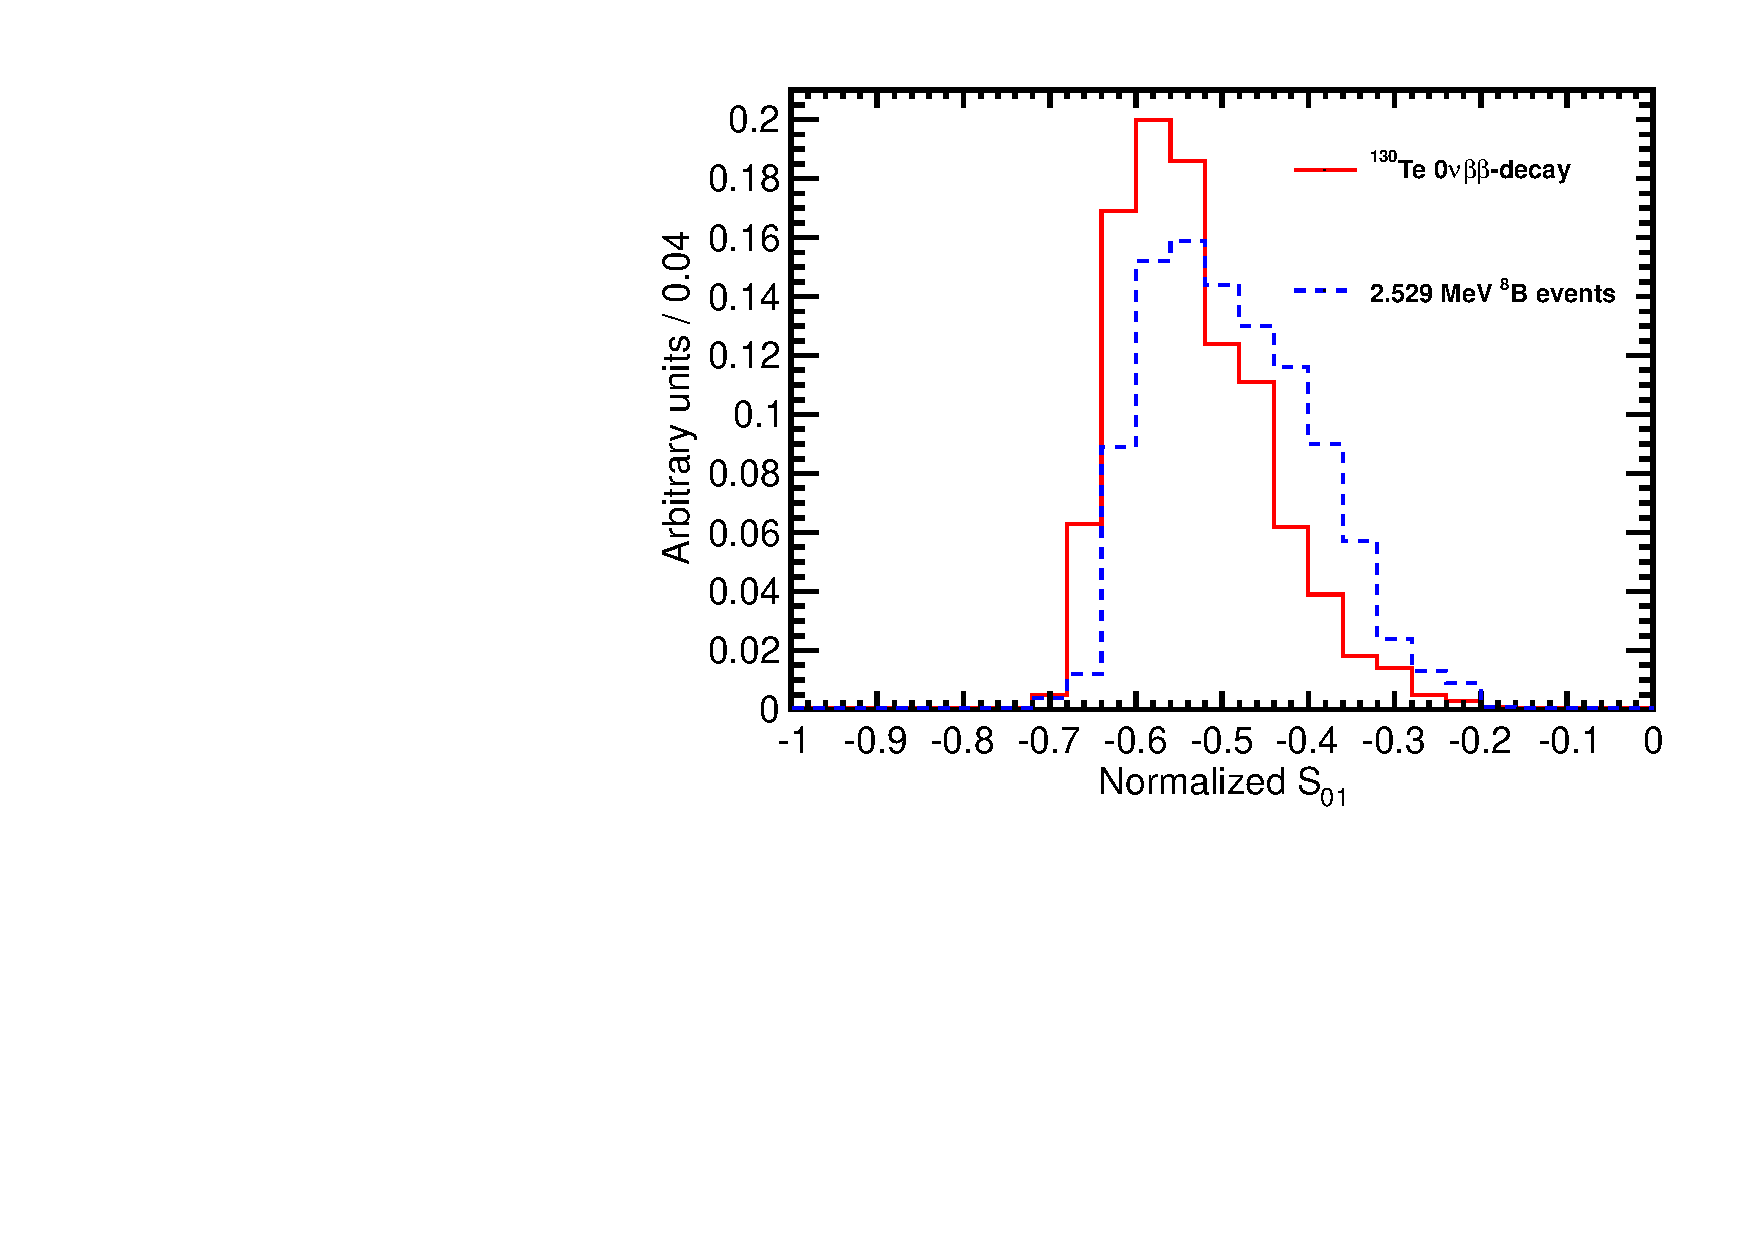
\includegraphics[width=0.49\textwidth]{hS01_allLight_VtxSmear3cm_VtxShiftX0cm_momDT1p0ns_rndVtx_3p0mSphere.pdf}
  \caption{Spherical harmonics comparison between $^{130}$Te 0{\nbb}
    decay signal ($Q=2.529$~MeV) (\emph{red}) and $^{8}$B solar
    neutrinos background (\emph{blue}) for 1000 simulated
    events.Verticies are uniformly distributed within the fiducial
    volume, R$<$3~m. $^8$Be events are implemented as 2.529~MeV
    electrons with the initial momentum direction uniformly
    distributed within 4$\pi$ solid angle. Vetrex is smeared with 3~cm
    resolution. \emph{Left:} $S_0$ versus $S_1$ scatter plot. Black
    dotted line is a linear fit of these 2D histograms. Variable
    $S_{01}$ is defined as a projection of 2D distribution onto this
    linear fit. \emph{Right:} $S_{01}$}
\label{fig:SL_Te_SmearX3cm_momDT1ns_rndVtx_3p0m}
\end{figure*}


{\bf Solution to this problem would be a better selection criteria of
  early light. It has to preserve high admixture of the Cherenkov
  photons, but needs to select scintillation photons in a more uniform
  manner. Working on it, but may not be simple so I don't want to
  include it in this paper.}

Good vertex resolution is essential for spherical harmonics analysis. As one can see in Fig.~\ref{fig:SL_Te_SmearX3cm_momDT1ns_rndVtx_3p0m}, even a 3~cm vertex resolution reduces the discrimination power of the spherical harmonics analysis.

Such strong dependence on the vertex resolution can be
addressed by choosing a different liquid scintillator mixture with a
more delayed emission of the scintillation light with respect to the Cherenkov light. With a larger delay in the scintillation light, a high fraction of Cherenkov light in the early PE sample selected with relative time cut $\Delta t$ can be maintained for a given vertex resolution. In addition, if the fraction of scintillation light is small compared to Cherenkov light, the distortions in the uniformity of the scintillation light distribution due to mis-reconstructed vertex do not significantly affect the $S_0$ and $S_1$ variables.

Figure~\ref{fig:SL_Te_momDT1ns_sci0p5ns_rndVtx_3p0m} shows
spherical harmonics analysis for the simulation where the
scintillation component is delayed by an additional 0.5ns compared to our default simulation. Events are simulated uniformly within the fiducial volume of the detector. Vertex resolution of 3~cm is assumed. Noticeable separation between $\vbb$ and $\B$ events is achieved.

The discrimination power of the spherical harmonics analysis improves with vertex resolution and more delay in the emission of the scintillation light. Moreover the dependence on vertex reconstruction reduces with delay in the scintillation light. 

\begin{figure*}[h]
  \centering
  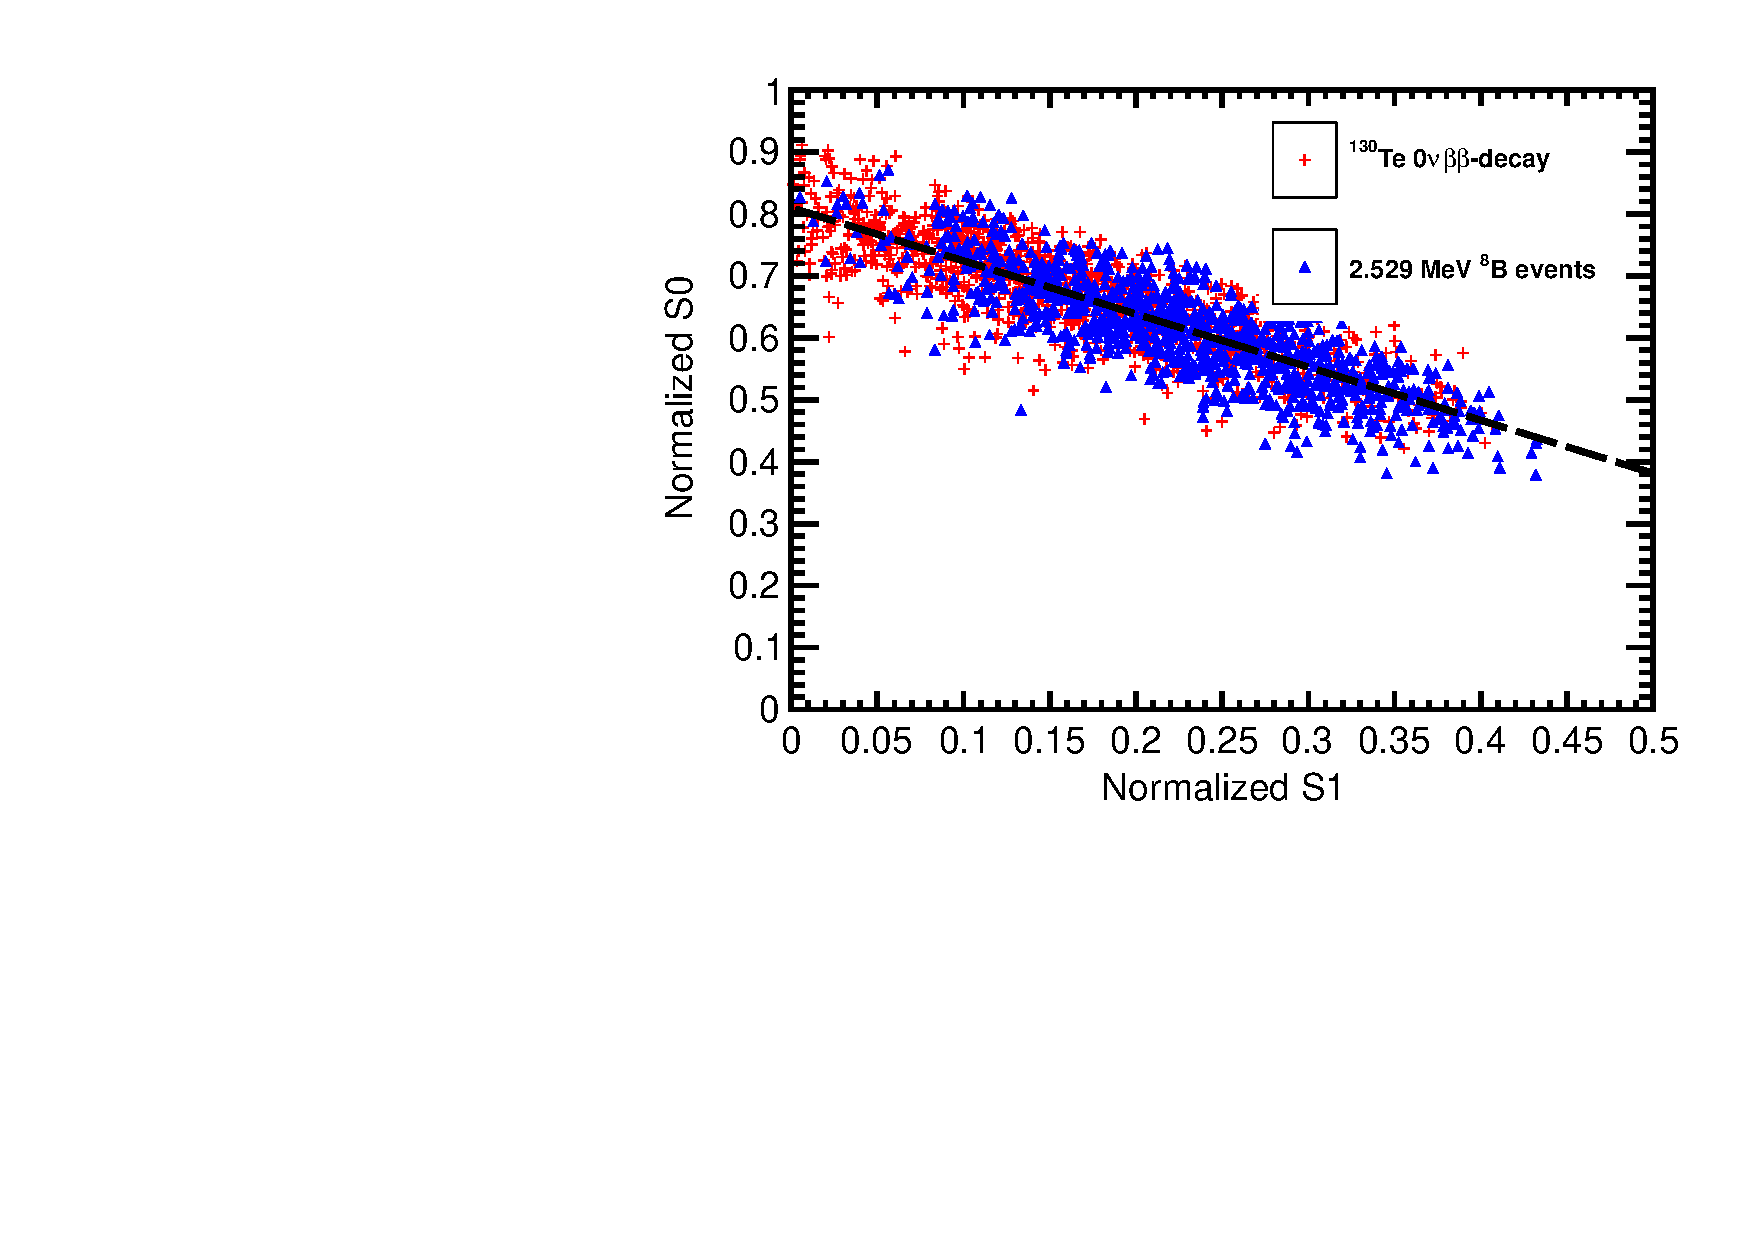
\includegraphics[width=0.49\textwidth]{hS0vsS1_Te130_1el_allLight_VtxSmear3cm_VtxShiftX0cm_momDT1p0ns_sci0p5ns_rndVtx_3p0mSphere.pdf}
  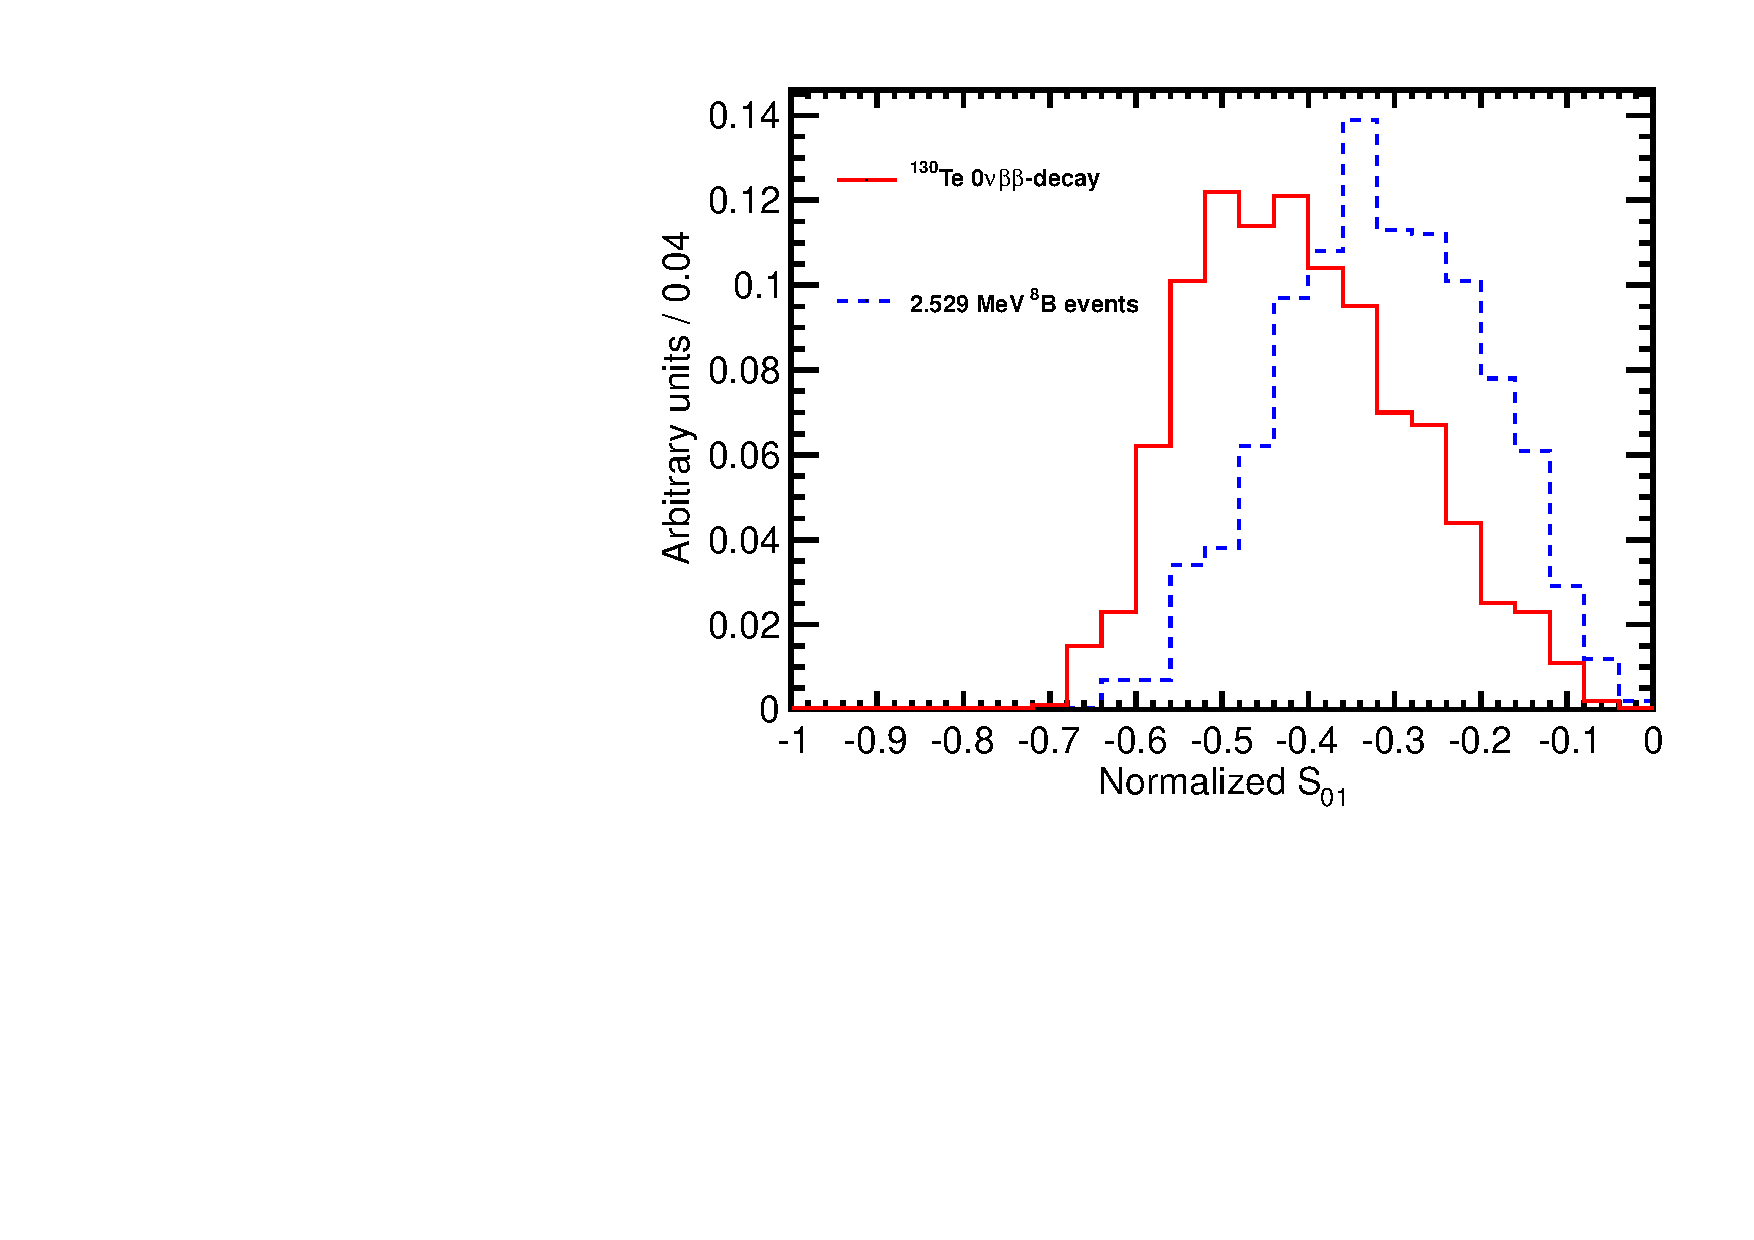
\includegraphics[width=0.49\textwidth]{hS01_allLight_VtxSmear3cm_VtxShiftX0cm_momDT1p0ns_sci0p5ns_rndVtx_3p0mSphere.pdf}
  \caption{Spherical harmonics comparison between $^{130}$Te 0{\nbb}
    decay signal ($Q=2.529$~MeV) (\emph{red}) and $^{8}$B solar
    neutrinos background (\emph{blue}) for 1000 simulated
    events. Verticies are uniformly distributed within the fiducial
    volume, $R<3$~m. $^8$Be events are implemented as 2.529~MeV
    electrons with the initial momentum direction uniformly
    distributed within 4$\pi$ solid angle. Vetrex is smeared with 3~cm
    resolution. {\bf Scintillation light is delayed by additional
      0.5~ns.} \emph{Left:} $S_0$ versus $S_1$ scatter plot. Black dotted
    line is a linear fit of these 2D histograms. Variable $S_{01}$ is
    defined as a projection of 2D distribution onto this linear
    fit. \emph{Right:} $S_{01}$}
\label{fig:SL_Te_SmearX3cm_momDT1ns_sci0p5ns_rndVtx_3p0m}
\end{figure*}

